\chapter{Implementación}
\section{Introducción}

En este capítulo se describirá la implementación del proyecto, dando énfasis en las tecnologías y dispositivos usados para el posicionamiento.

\section{Implementación general de trabajo}
A continuación se observa el esquema general del algoritmo a implementar y cómo confluyen ambas partes para llevar a cambo el posicionamiento.

\begin{figure}[h!]
    \centering
    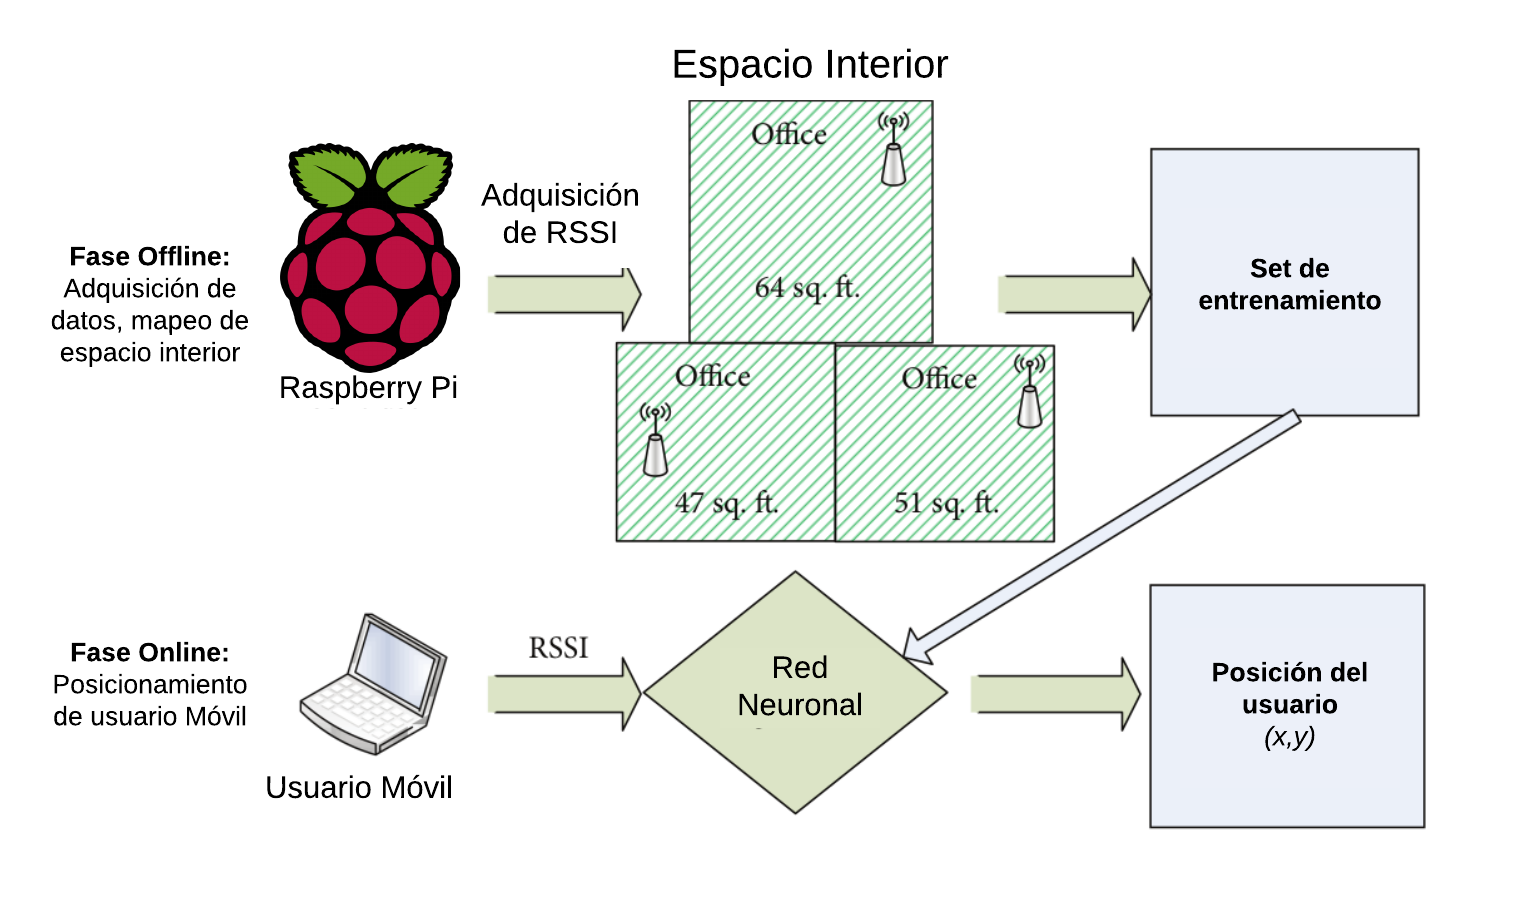
\includegraphics[scale=0.6]{./images/esquema}
    \caption{Esquema de Implementación General de Trabajo}
    \label{fig:esquema2}
\end{figure}

\subsection{Adquisición de RSSI}
La adquisición de estos datos se hará con la librería de linux llamada \texttt{iwlist}. Una breve descripción de esta, a continuación:
\begin{itemize}
    \item {\textbf{Descripción}: Iwlist es usada para mostrar información adicional de dispositivos inalámbricos de una red. El argumento principal es usada para seleccionar una categoría de información, \texttt{iwlist} muestra información en detalle para toda la información relacionada a esta categoría, incluyendo la información que se muestra en \texttt{iwconfig}.\\}
    
    \item {\texttt{scan[ning]}: Entrega una lista completa de los Access Points y celdas Ad-Hoc en el rango, y opcionalmente, información adicional sobre ellos. Algunos de estos datos adicionales son \texttt{ESSID, Quality, Frequency, Mode, etc} que permiten entre otras cosas, reconocer la \textbf{dirección MAC} de los dispositivos, el \textbf{RSSI}, y el \textbf{nombre de la red}.
    
    En esta parte, es necesario recalcar que las características a desplegar dependerán de la tarjeta de red de manera que para efectos del proyecto, se limitarán a la tarjeta del computador en uso.\\
    }
    \begin{figure}[h!]
        \centering
        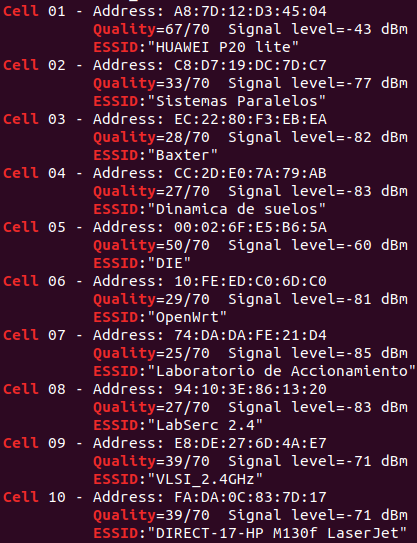
\includegraphics[scale=0.4]{./images/output}
        \caption{Salida de consola con datos de AP}
        \label{fig:output}
    \end{figure}
    
    A través de esta opción, y haciendo uso de la Raspberry Pi facilitada por la carrera, se puede hacer un mapeo de cómo, para una posición específica, sea por ejemplo $(x,y) = (0,0)$ el punto de origen de las mediciones, y obtener así las medidas para cada punto en el plano, llevando así a cabo, la caracterización del espacio mencionada en \ref{fig:esquema}.
\end{itemize}

\newpage

Las mediciones se harán en espacio accesible, esto es, pasillo del segundo piso del edificio Tecnológico Mecánico a una distancia de separación entre un punto y otro de 50 cm, allí se posicionará la Raspberry sobre un trípode y se pondrá a medir durante 15 segundos por cada una de las distintas orientaciones, esto es, izquierda, derecha, adelante y atrás. De este modo, se tiene una caracterización espacial del plano por el cual se moverán los objetivos.\\

% \begin{figure}[h!]
%     \centering
%     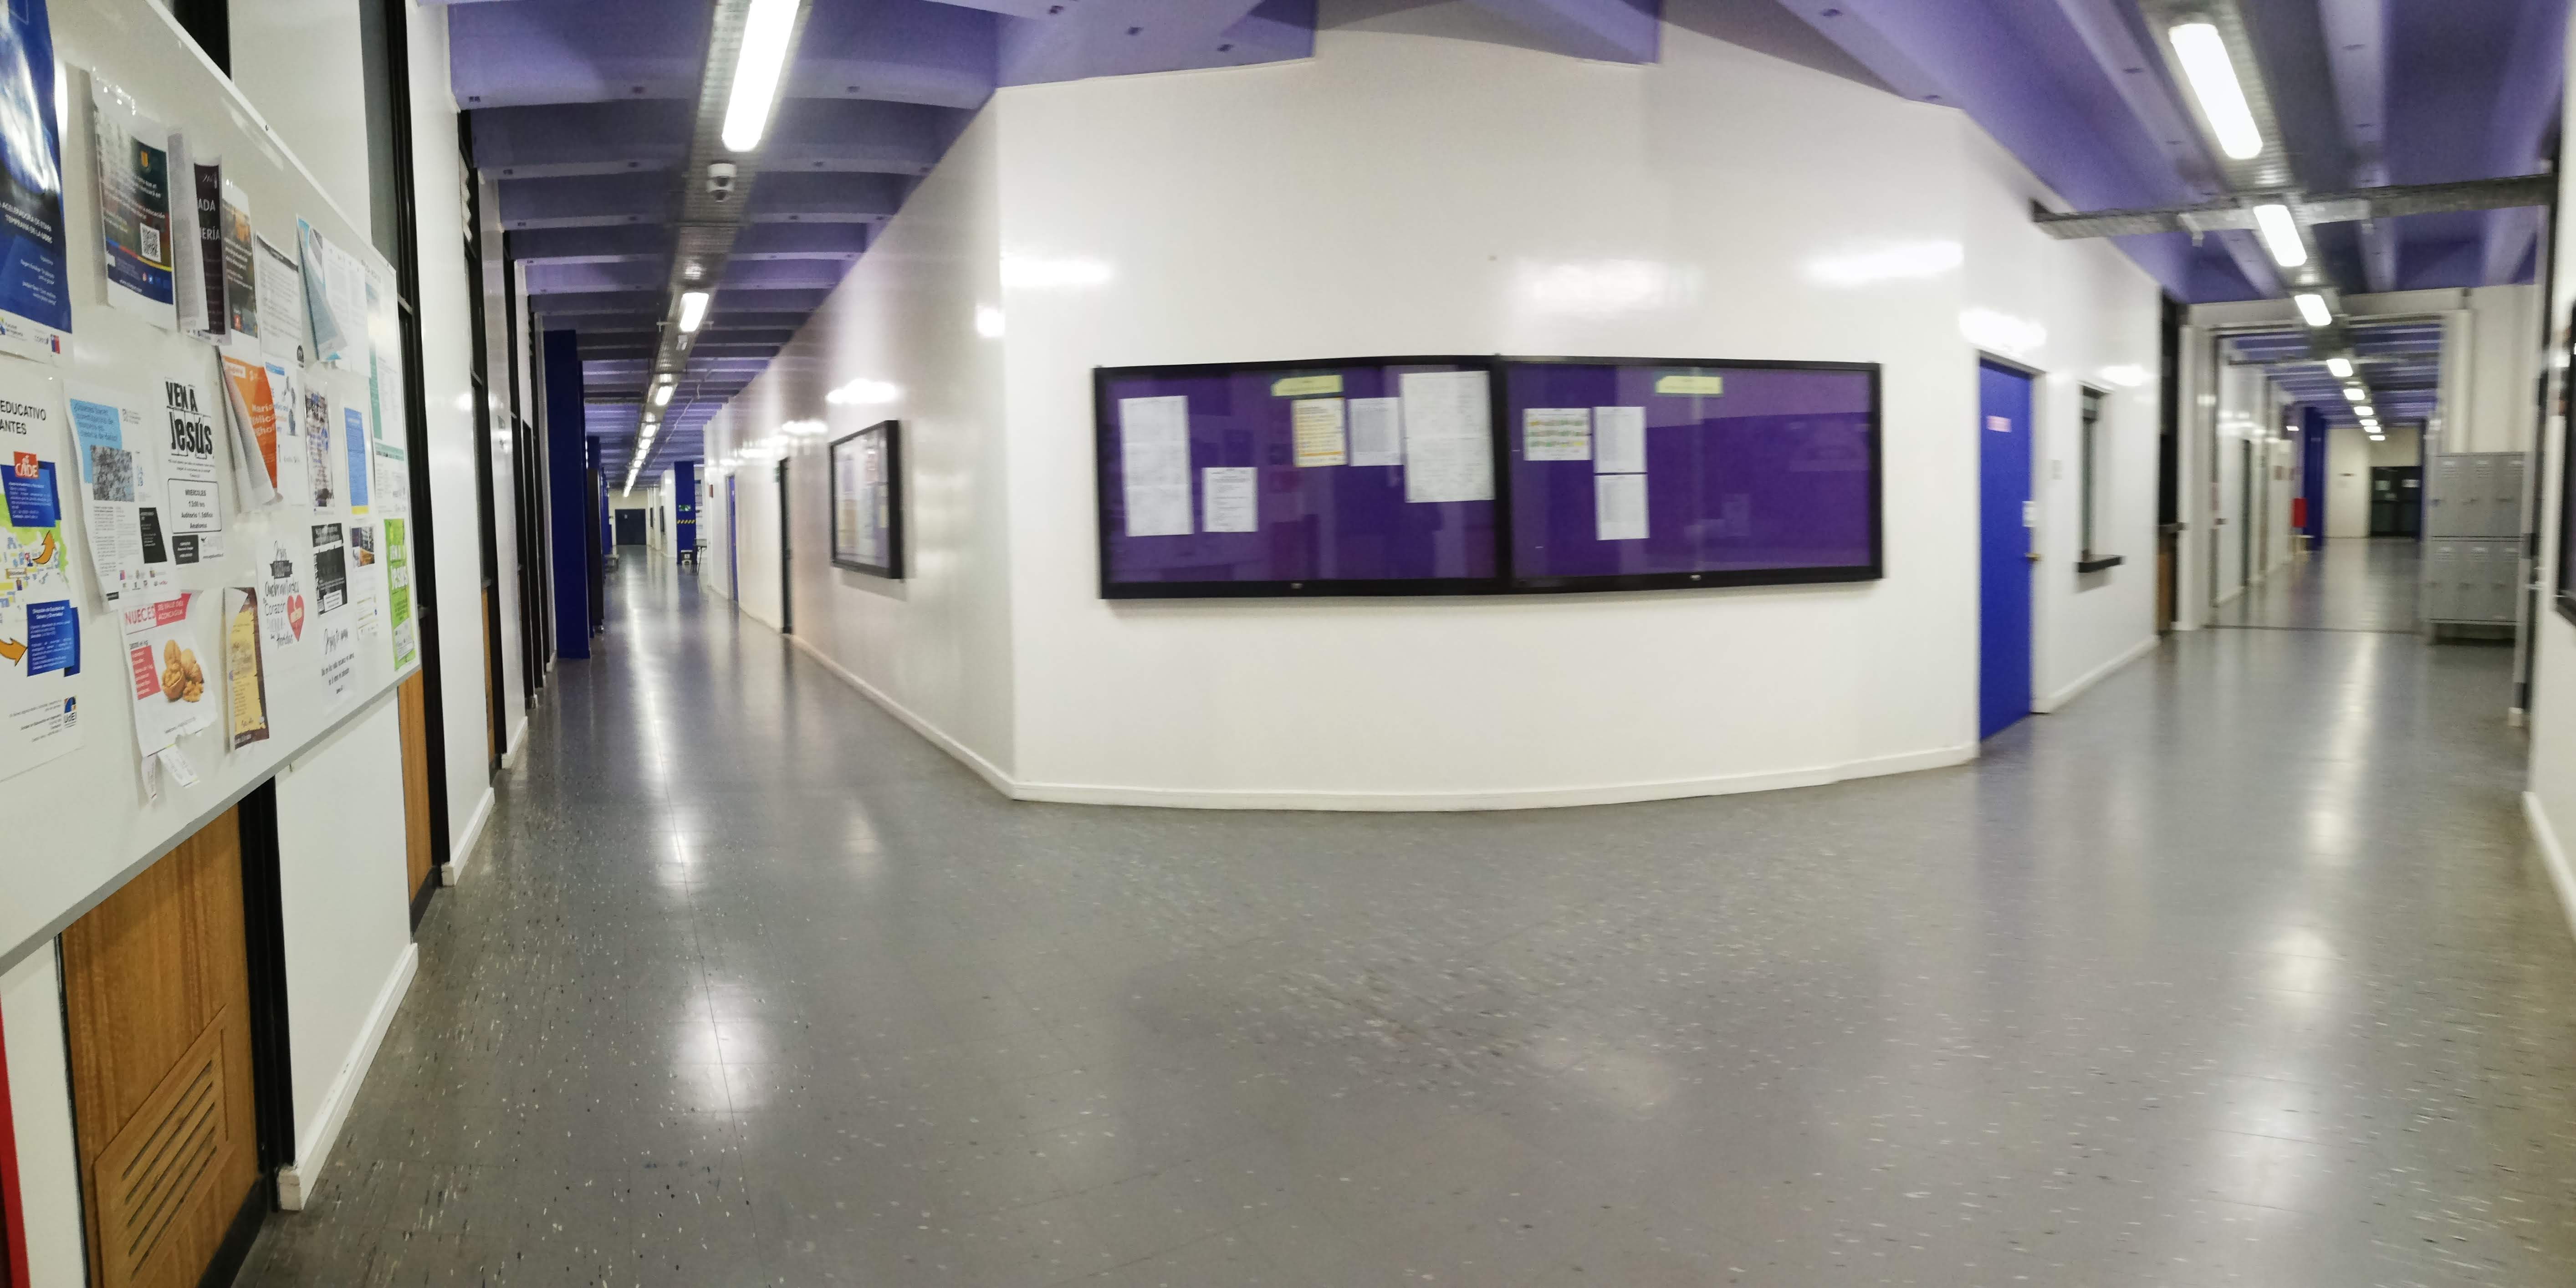
\includegraphics[scale=0.4]{./imagenes/pasillo}
%     \caption{Segundo piso Edificio Tecnológico Mecánico}
%     \label{fig:2do}
% \end{figure}

\subsection{Set de entrenamiento}
En esta parte, los datos son filtrados, separados y agrupados en un archivo csv para la posterior lectura y procesamiento de la Red Neuronal.\\

El formato de los datos de entrega es el siguiente.
\begin{figure}[h!]
    \centering
    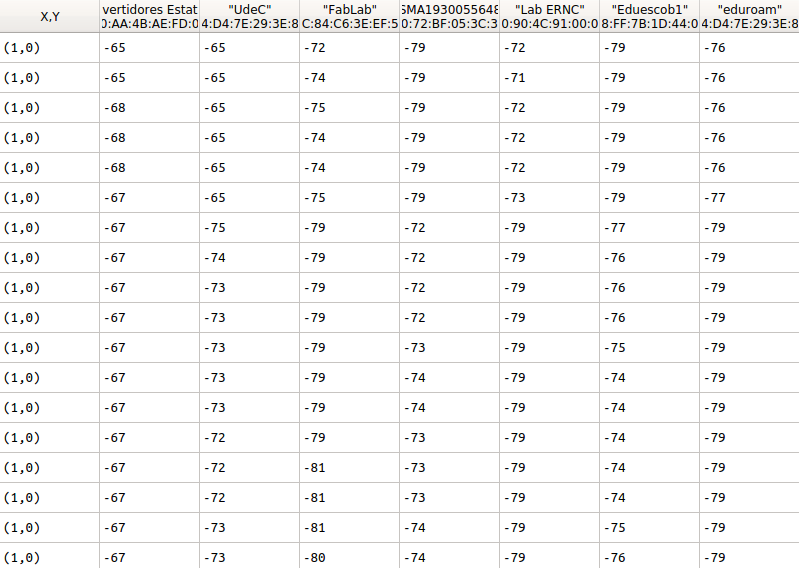
\includegraphics[scale=0.5]{./images/datos}
    \caption{Formato tipo de datos entregados }
    \label{fig:datos}
\end{figure}

Del cual, la información relevante sólo es la potencia recibida de modo que se pueden prescindir de los demás datos a la hora de hacer de estos las input de la red.

\subsubsection{Red Neuronal}
La Red Neuronal es fundamental para el posicionamiento del objetivo, se compone a priori, de 10 nodos o neuronas, en la capa de entrada, 6 y 4 en las capas ocultas y 1 en la capa de salida.\\

\begin{figure}[h!]
    \centering
    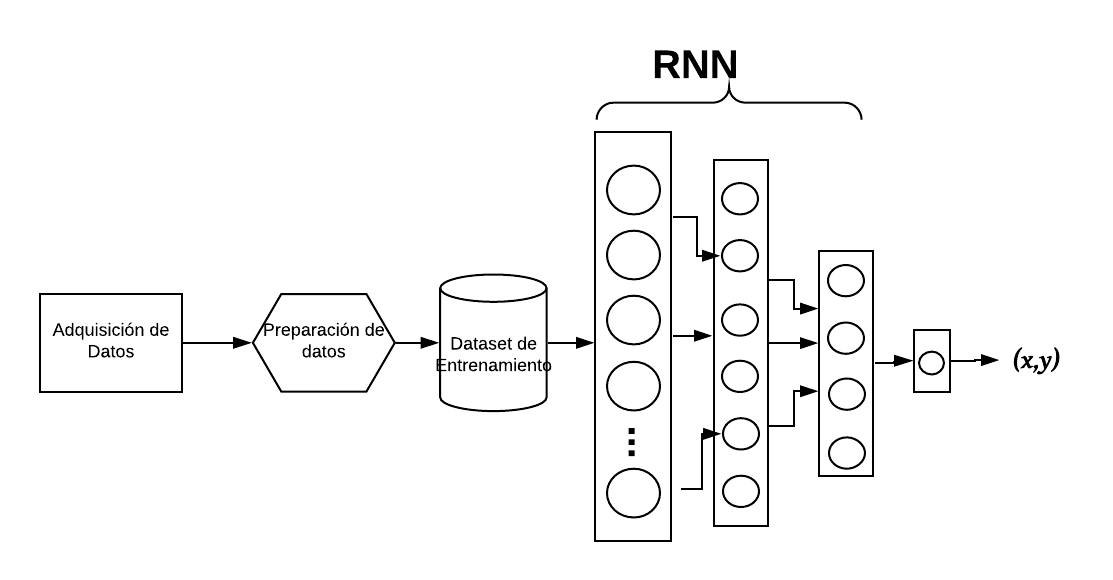
\includegraphics[scale=0.4]{./images/Red_offline}
    \caption{Diagrama de funcionamiento de procehttps://www.overleaf.com/project/5cf12ec0c55efb56ff0b453bso offline}
    \label{fig:Red_offline}
\end{figure}

Esta será implementada usando la biblioteca de redes neuronales \texttt{Keras}, la cual es biblioteca de Redes Neuronales OpenSource escrita en Python, capaz de ejecutarse sobre TensorFlow, Microsoft Cognitive Toolkit o Theano.\\

Está diseñada para facilitar la experimentación con redes de Deep Learning en corto plazo. Se caracteriza por ser amigable para el usuario, modular y extensible.

\newpage
\subsection{Visualización de Posición del Usuario}

